\documentclass[border=3pt,tikz]{standalone}
\usepackage{amsmath}
\usetikzlibrary{calc}
\usetikzlibrary{arrows.meta} % for arrow size
\begin{document}
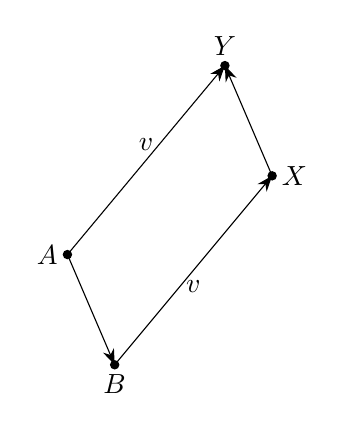
\begin{tikzpicture}[scale=2]
\usetikzlibrary {arrows.meta}
\usetikzlibrary {calc}

\coordinate (A) at (0,0);
\coordinate (Y) at (1,1.2);
\coordinate (B) at (0.3, -0.7);
\coordinate (X) at (1.3, 0.5);
\draw[black, -{Stealth[length=2mm]}] (A) -- node[above] {$v$}  (Y);
\draw[black, -{Stealth[length=2mm]}] (A) -- (B);
\draw[black, -{Stealth[length=2mm]}] (B) -- node[below] {$v$} (X);
\draw[black, -{Stealth[length=2mm]}] (X) -- (Y);
\fill[black] (A) circle (0.03cm) node[left] {$A$};
\fill[black] (X) circle (0.03cm) node[right] {$X$};
\fill[black] (B) circle (0.03cm) node[below] {$B$};
\fill[black] (Y) circle (0.03cm) node[above] {$Y$};


\end{tikzpicture}
\end{document}